\chapter{Schéma a návrh \acs{dps} řídicí jednotky}
	\label{priloha:schema-a-dps-ridici-jednotka}
	\section{Blokové schéma}
	\label{priloha:schema-ridici-jednotka-blokove}
		% trim=left bottom right top
		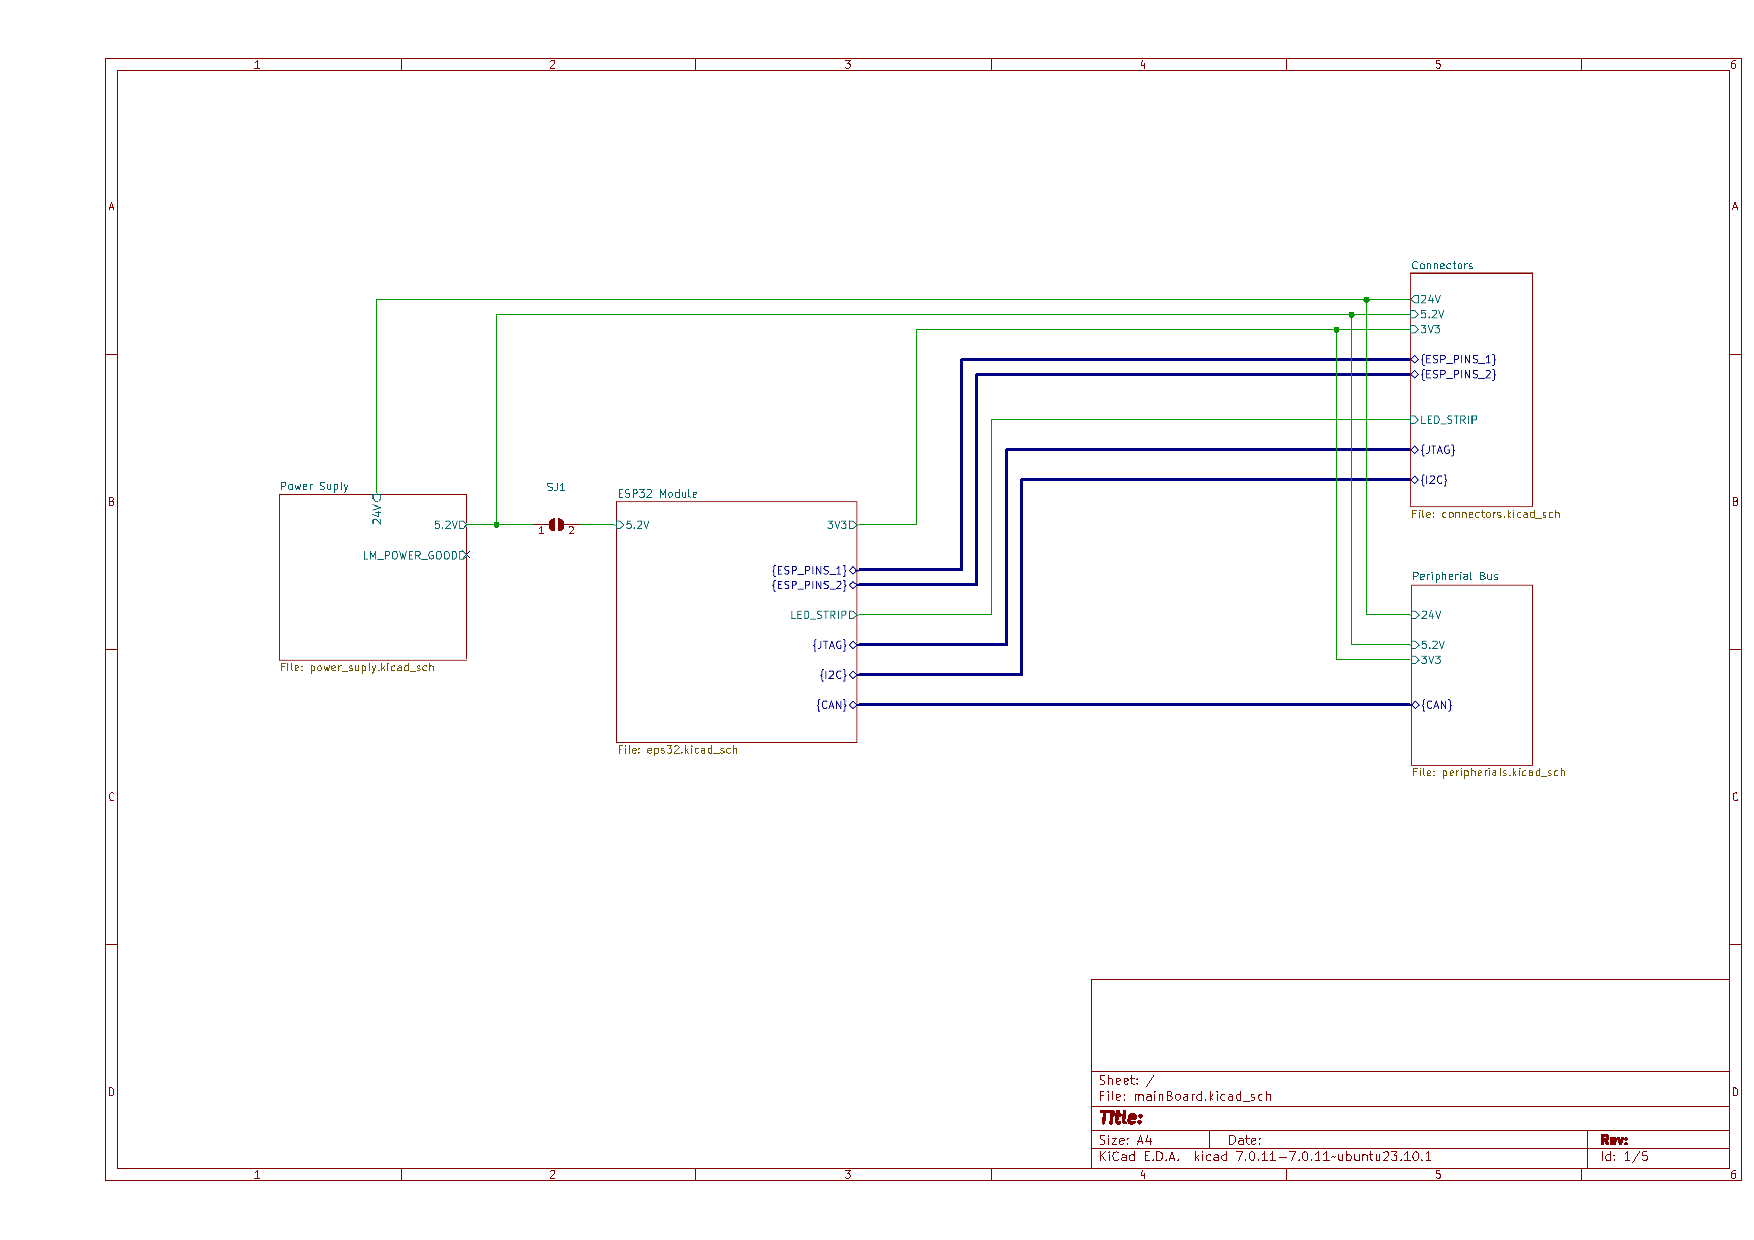
\includegraphics
		[
			width=\textheight, height=0.9\textwidth, keepaspectratio,
			page=1, 
			angle=90,
			trim=1.5cm 1cm 0cm 1cm, 
			clip
		]{obrazky/exportovane/main-board-schematic.pdf}

	\section{Zapojení \acs{mcu}}
	\label{priloha:schema-ridici-jednotka-mcu}
		% trim=left bottom right top
		\includegraphics
		[
			width=\textheight, height=\textwidth, keepaspectratio,
			page=2, 
			angle=90,
			trim=1.5cm 1cm 0cm 1cm, 
			clip
		]{obrazky/exportovane/main-board-schematic.pdf}

	\section{Napájecí obvod}
	\label{priloha:schema-ridici-jednotka-napajeci-obvod}
		% trim=left bottom right top
		\includegraphics
		[
			width=\textheight, height=\textwidth, keepaspectratio,
			page=3, 
			angle=90,
			trim=1.5cm 1cm 0cm 1cm, 
			clip
		]{obrazky/exportovane/main-board-schematic.pdf}

	\section{Konektory}
	\label{priloha:schema-ridici-jednotka-konektory}
		% trim=left bottom right top
		\includegraphics
		[
			width=\textheight, height=\textwidth, keepaspectratio,
			page=4, 
			angle=90,
			trim=1.5cm 1cm 0cm 1cm, 
			clip
		]{obrazky/exportovane/main-board-schematic.pdf}

	\section{Sběrnice periferií}
	\label{priloha:schema-ridici-jednotka-periferie}
		% trim=left bottom right top
		\includegraphics
		[
			width=\textheight, height=\textwidth, keepaspectratio,
			page=5, 
			angle=90,
			trim=1.5cm 1cm 0cm 1cm, 
			clip
		]{obrazky/exportovane/main-board-schematic.pdf}
	
	\section{Vodivé motivy \acs{dps}}
	\label{priloha:dps-main-board}
		\begin{tikzpicture}
			% Define the width of each image
			\newcommand{\imagewidth}{0.45\linewidth}
			\newcommand{\rowheight}{0.75\linewidth}
			\newcommand{\pdffilepath}{obrazky/exportovane/mainBoardDPS/color.pdf}
			% \newcommand{\pdffilepath}{obrazky/exportovane/mainBoardDPS/bw.pdf} %BW version
		
			% Row 1
			\node[anchor=south west,inner sep=0, label={[align=center]Vodivý motiv horní strany \\(F.Cu)}] at (0, 0) {\includegraphics[page=1,width=\imagewidth]{\pdffilepath}};
			\node[anchor=south west,inner sep=0, label={[align=center]Vodivý motiv spodní strany\\(B.Cu)}] at (\imagewidth, 0) {\includegraphics[page=4,width=\imagewidth]{\pdffilepath}};
		
			% Row 2
			\node[anchor=south west,inner sep=0, label={[align=center]Vodivý motiv 1. vnitřní vrstvy\\(In1.Cu)}] at (0, -\rowheight) {\includegraphics[page=2,width=\imagewidth]{\pdffilepath}};
			\node[anchor=south west,inner sep=0, label={[align=center]Vodivý motiv 2. vnitřní vrstvy\\(In2.Cu)}] at (\imagewidth, -\rowheight) {\includegraphics[page=3,width=\imagewidth]{\pdffilepath}};
		\end{tikzpicture}


\chapter{Schéma a návrh \acs{dps} modulu periferií}
\label{priloha:schema-a-dps-modul-periferii}
\section{Vodivé motivy \acs{dps}}
\label{priloha:dps-modul-periferii}
	\begin{tikzpicture}
		% Define the width of each image
		\newcommand{\imagewidth}{0.48\linewidth}
		\newcommand{\rowheight}{0.65\linewidth}
		\newcommand{\pdffilepath}{obrazky/exportovane/peripherialModuleDPS/color.pdf}
		% \newcommand{\pdffilepath}{obrazky/exportovane/mainBoardDPS/bw.pdf} %BW version

		% Row 1
		\node[anchor=south west,inner sep=0, label={[align=center]Vodivý motiv horní strany \\(F.Cu)}] at (0, 0) {\includegraphics[trim=0cm 4cm 0cm 4cm, page=1,width=\imagewidth]{\pdffilepath}};
		\node[anchor=south west,inner sep=0, label={[align=center]Vodivý motiv spodní strany\\(B.Cu)}] at (\imagewidth, 0) {\includegraphics[trim=0cm 4cm 0cm 4cm, page=4,width=\imagewidth]{\pdffilepath}};

		% Row 2
		\node[anchor=south west,inner sep=0, label={[align=center]Vodivý motiv 1. vnitřní vrstvy\\(In1.Cu)}] at (0, -\rowheight) {\includegraphics[trim=0cm 4cm 0cm 4cm, page=2,width=\imagewidth]{\pdffilepath}};
		\node[anchor=south west,inner sep=0, label={[align=center]Vodivý motiv 2. vnitřní vrstvy\\(In2.Cu)}] at (\imagewidth, -\rowheight) {\includegraphics[trim=0cm 4cm 0cm 4cm, page=3,width=\imagewidth]{\pdffilepath}};
	\end{tikzpicture}


	\section{Schéma zapojení}
	\label{priloha:schema-modul-periferii}
		% trim=left bottom right top
		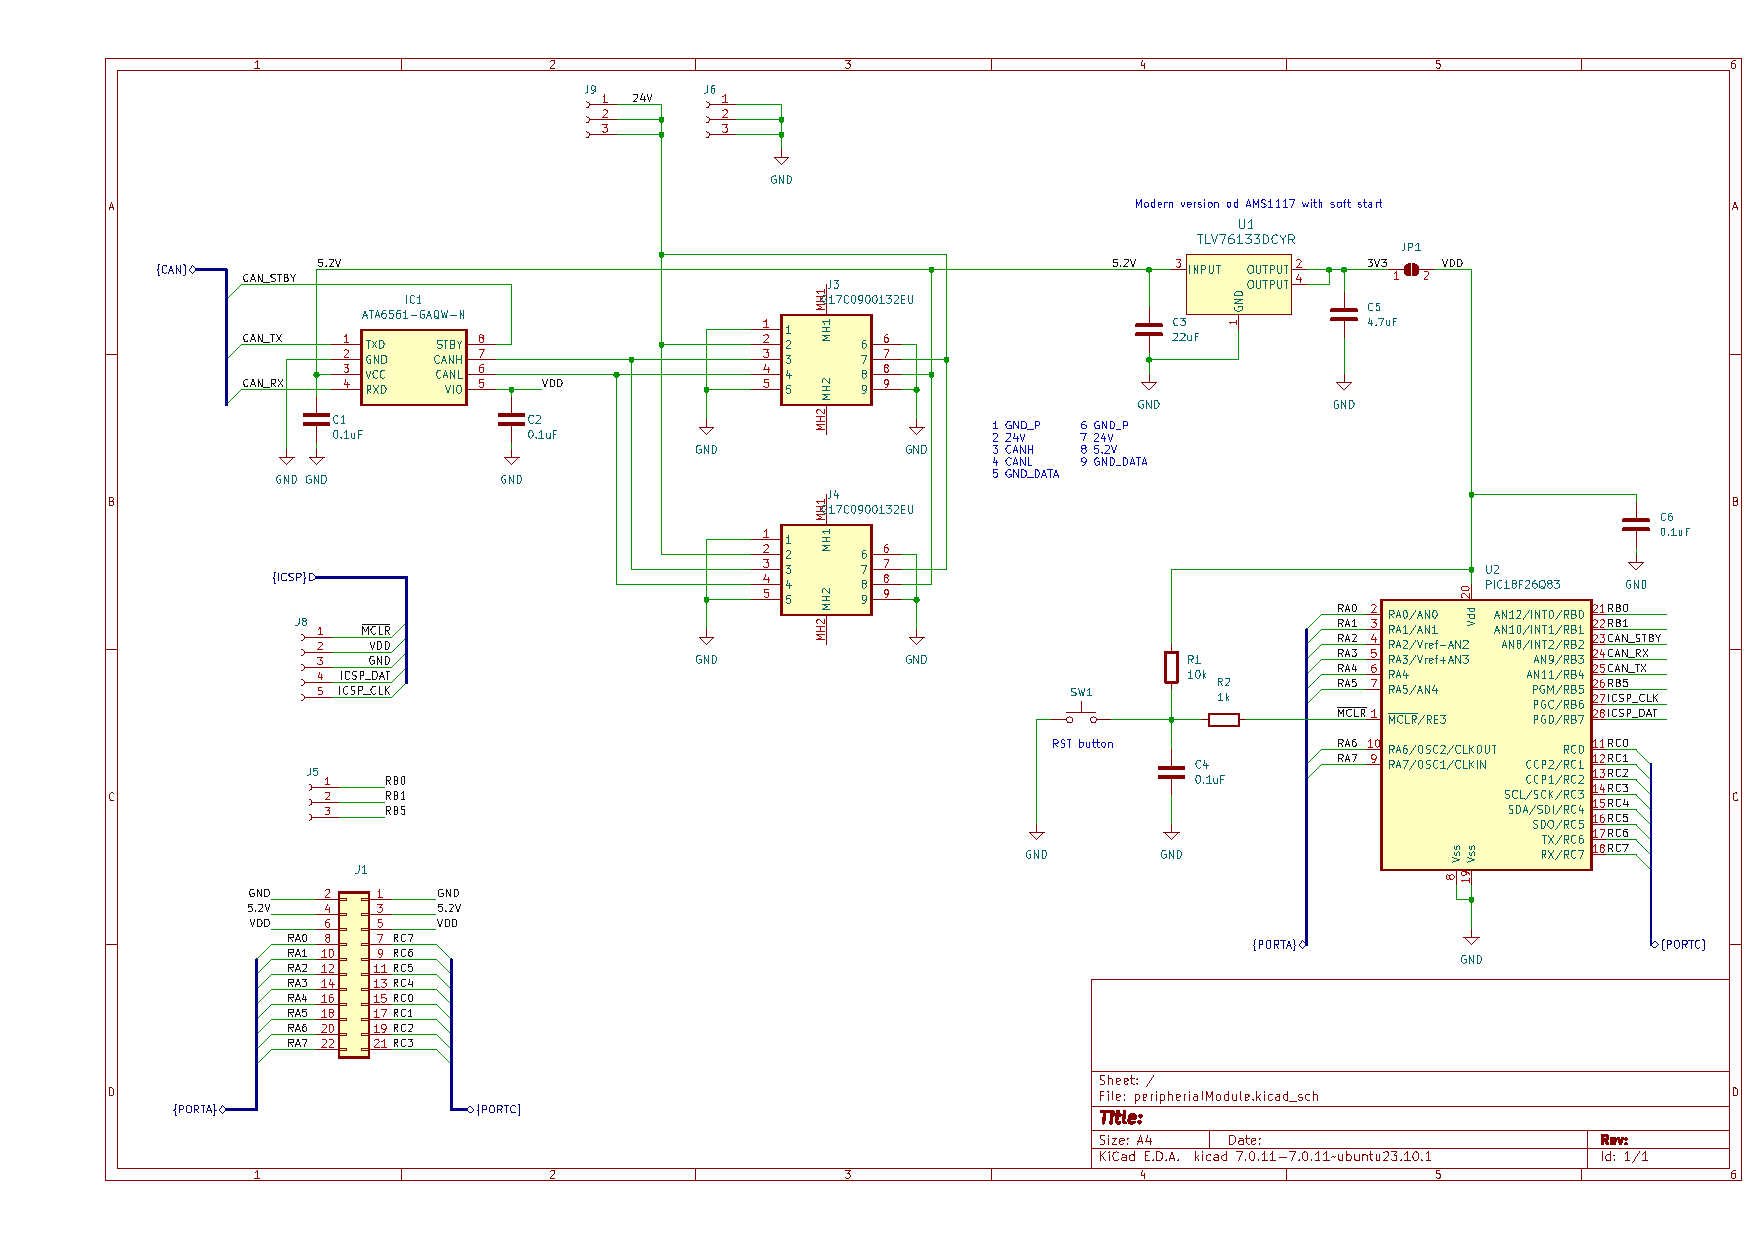
\includegraphics
		[
			width=\textheight, height=\textwidth, keepaspectratio,
			page=1, 
			angle=90,
			trim=1.5cm 1cm 0cm 1cm, 
			clip
		]{obrazky/exportovane/peripherial-module-schematic.pdf}

	
\chapter{Schéma a návrh \acs{dps} modulu \acs{led} osvětlení}
\label{priloha:schema-a-dps-led-board}

\section{Vodivé motivy \acs{dps}}
\label{priloha:dps-led-board}
\begin{tikzpicture}
	% Define the width of each image
	\newcommand{\imagewidth}{0.48\linewidth}
	\newcommand{\rowheight}{0.5\linewidth}
	\newcommand{\pdffilepath}{obrazky/exportovane/ledBoardDPS/color.pdf}
	% \newcommand{\pdffilepath}{obrazky/exportovane/mainBoardDPS/bw.pdf} %BW version
	
	% Row 1
	\node[anchor=south west,inner sep=0, label={[align=center]Vodivý motiv horní strany \\(F.Cu)}] at (0, 0) {\includegraphics[page=1,width=\imagewidth]{\pdffilepath}};
	\node[anchor=south west,inner sep=0, label={[align=center]Vodivý motiv spodní strany\\(B.Cu)}] at (\imagewidth, 0) {\includegraphics[page=4,width=\imagewidth]{\pdffilepath}};
	
	% Row 2
	\node[anchor=south west,inner sep=0, label={[align=center]Vodivý motiv 1. vnitřní vrstvy\\(In1.Cu)}] at (0, -\rowheight) {\includegraphics[page=2,width=\imagewidth]{\pdffilepath}};
	\node[anchor=south west,inner sep=0, label={[align=center]Vodivý motiv 2. vnitřní vrstvy\\(In2.Cu)}] at (\imagewidth, -\rowheight) {\includegraphics[page=3,width=\imagewidth]{\pdffilepath}};
\end{tikzpicture}

\section{Schéma zapojení}
\label{priloha:schema-led-board}
% trim=left bottom right top
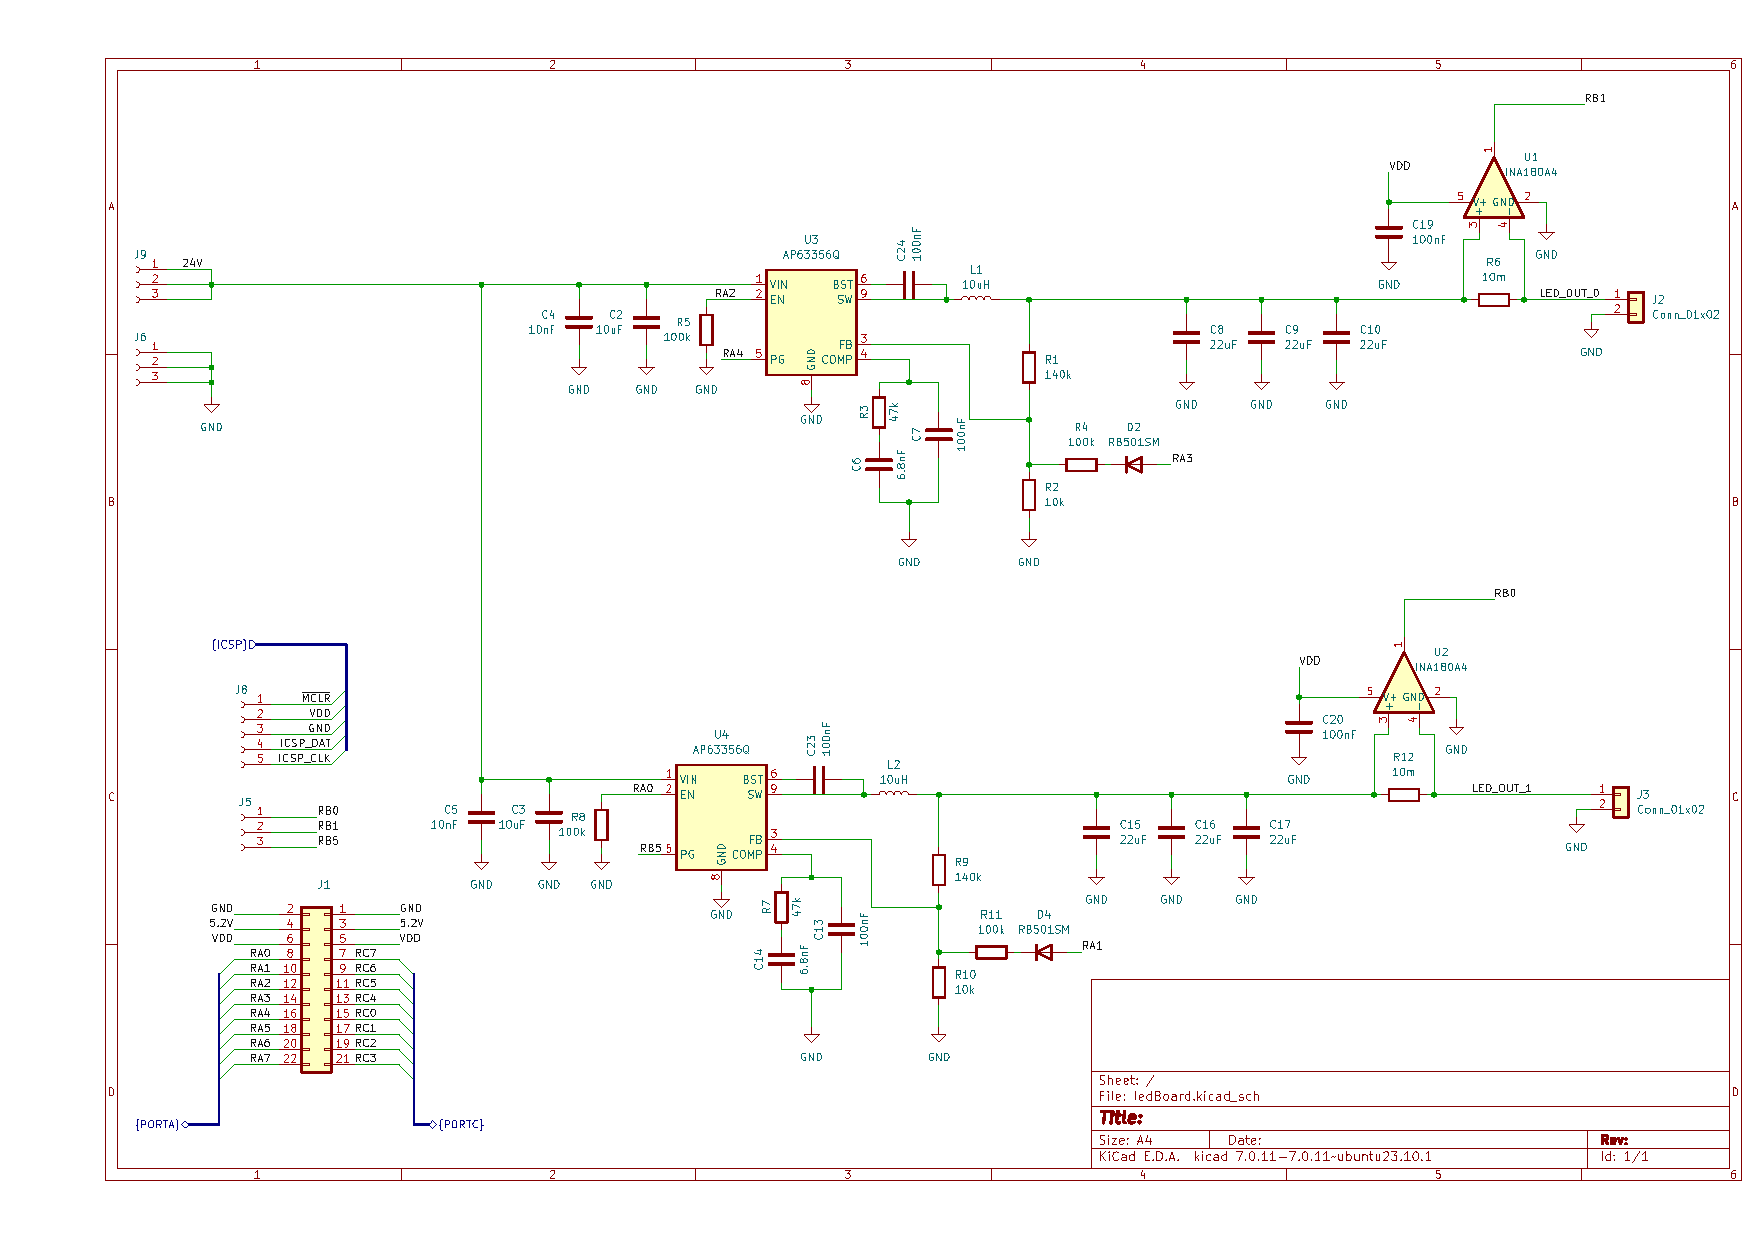
\includegraphics
[
	width=\textheight, height=\textwidth, keepaspectratio,
			page=1, 
			angle=90,
			trim=1.5cm 1cm 0cm 1cm, 
			clip
		]{obrazky/exportovane/led-board-schematic.pdf}
		